\section{相关工作}
\subsection{BEV 3D目标检测器}
鸟瞰视图（BEV）目标检测（Object Detection）近年来受到越来越多的关注~\cite{OFT,VPN,pseudo-lidar,LSS,bevformer,CVT,PETR}，在自动驾驶系统中取得了巨大成功。

早期工作包括 OFT~\cite{OFT}、Pseudo LiDAR~\cite{pseudo-lidar} 和 VPN~\cite{VPN}，它们揭示了如何将透视图特征转换为BEV特征，但要么仅针对单摄像头，要么在不太知名的任务上评估。
OFT~\cite{OFT} 率先采用从2D图像特征到3D BEV特征的转换用于单目3D目标检测（Monocular 3D Object Detection）。
Pseudo LiDAR~\cite{pseudo-lidar} 顾名思义，通过单目深度估计（Monocular Depth Estimation）和相机内参创建伪点云，随后在BEV空间中进行处理。
VPN~\cite{VPN} 首次将多视角（Multi-view）相机输入融合为俯视图特征图用于语义分割（Semantic Segmentation）。

现代方法充分利用了2D-3D视图变换（View Transformation）提供的从不同透视图传感器整合特征的便利。
LSS~\cite{LSS} 通过引入潜在深度分布（Latent Depth Distribution）扩展了 OFT，用于BEV柱状特征的池化。此外，LSS 对六个环绕图像（而非 OFT 中的单张图像）进行了池化。
与 LSS 的2D到3D提升或 OFT 的3D到2D投影不同，CVT~\cite{CVT} 利用相机感知位置编码（Camera-aware Positional Encoding）和密集交叉注意力（Dense Cross Attention）连接透视图和BEV视图的特征。
PETR~\cite{PETR} 设计了一种无需显式BEV特征构建的方法，将透视图特征图与3D位置嵌入特征图逐元素融合，然后应用 DETR 风格的解码器（Decoder）进行目标检测。
BEVFormer~\cite{bevformer} 利用空间交叉注意力（Spatial Cross-attention）进行视图变换和时序自注意力（Temporal Self-attention）进行时序特征融合。BEVFormer 完全基于 Transformer 的结构使其BEV特征比其他方法更通用，能够轻松支持非均匀和非规则的采样网格。
此外，如 SimpleBEV~\cite{simplebev} 所示，多尺度可变形注意力（Multi-scale Deformable Attention）~\cite{deformable-detr} 在所有提升策略中表现最佳。
因此，本文选择基于 BEVFormer 构建检测器以利用上述优势。

除已发表的工作外，由于该领域的受欢迎程度，还有许多同期工作。
BEVDet~\cite{BEVDet} 引入了丰富的图像级和BEV级数据增强用于训练。
BEVStereo~\cite{bevstereo} 和 STS~\cite{STS} 均采用时序立体（Temporal Stereo）范式以获得更好的深度估计。
PolarFormer~\cite{polarformer} 提出了非笛卡尔（Non-cartesian）3D网格设置。
SimpleBEV~\cite{simplebev} 比较了不同的2D-3D提升方法。

与现有主要探索检测器设计的工作不同，本文专注于将现代图像骨干网络适配到BEV识别模型中。

\begin{figure*}[t]
    \centering
    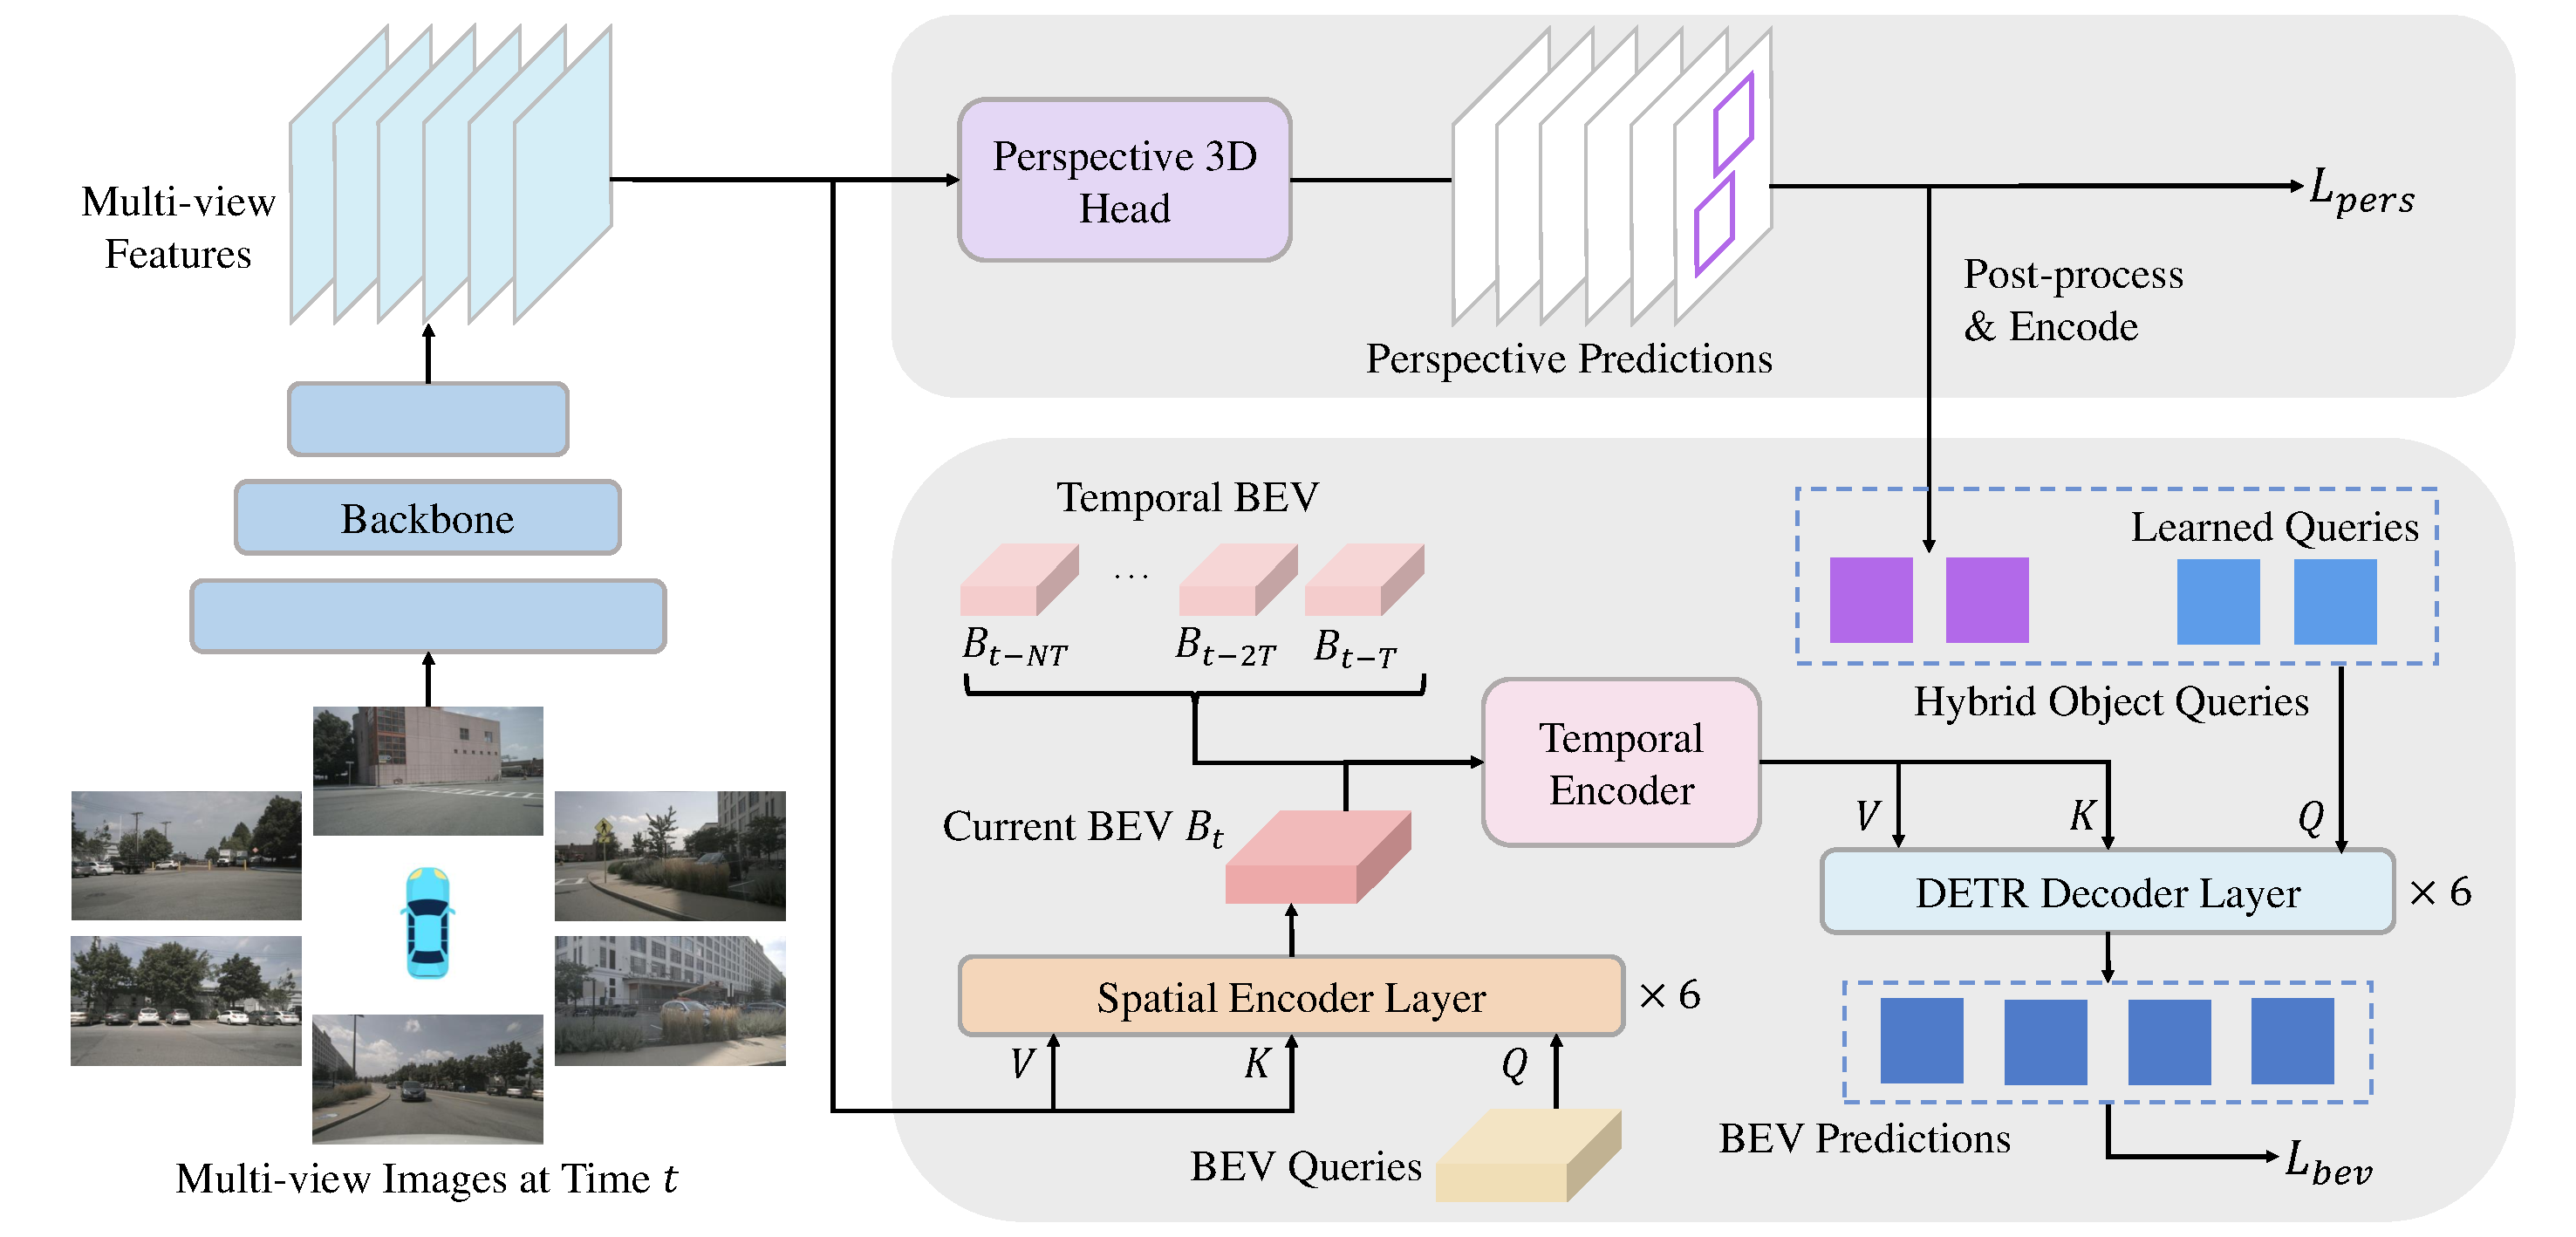
\includegraphics[width=0.9\textwidth]{figures/architecture2.pdf}
    \caption{BEVFormer v2 的整体架构。图像骨干网络提取多视角图像特征。透视3D头生成透视图预测，随后编码为物体查询（Object Query）。BEV头采用编码器-解码器（Encoder-Decoder）结构。空间编码器（Spatial Encoder）通过聚合多视角图像特征生成BEV特征，时序编码器（Temporal Encoder）收集历史BEV特征。解码器以混合物体查询（Hybrid Object Query）为输入，基于BEV特征生成最终BEV预测。整个模型使用两个检测头的损失项 $L_{pers}$ 和 $L_{bev}$ 进行训练。}
    \label{fig:architecture}
\end{figure*}

\subsection{相机3D目标检测中的辅助损失}
辅助损失（Auxiliary Loss）在单目3D目标检测中无处不在，因为大多数方法~\cite{MonoDIS,monoflex,fcos3d,DD3D,MonoCon,bevdepth,mv-fcos3d} 都建立在 RetinaNet~\cite{RetinaNet} 和 FCOS~\cite{fcos} 等2D检测器之上。
但这些辅助损失很少赋予2D监督任何明确的含义。
MonoCon~\cite{MonoCon} 充分利用了2D辅助损失，使用了多达5种不同的2D监督。
对于BEV检测器，BEVDepth~\cite{bevdepth} 利用 LiDAR 点云监督其中间深度网络。
MV-FCOS3D++~\cite{mv-fcos3d} 引入了透视监督（Perspective Supervision）用于训练其图像骨干网络，但检测器本身仅由BEV损失监督。
SimMOD~\cite{SimMOD} 为其单目提议头（Monocular Proposal Head）使用了2D辅助损失。

与先前方法不同，本文采用了端到端（End-to-end）的透视监督方法，无需使用 LiDAR 点云等额外数据。

\subsection{两阶段3D目标检测器}
尽管两阶段（Two-stage）检测器在基于 LiDAR 的3D目标检测中很常见~\cite{MV3D,AVOD,centerpoint,lidar-rcnn,frustum-pointnet,transfusion,SimMOD}，但其在基于相机的3D检测中的应用却鲜为人知。
MonoDIS~\cite{MonoDIS} 使用 RoIAlign 从2D框中提取图像特征并随后回归3D框。
SimMOD~\cite{SimMOD} 使用单目3D头生成提议，并使用 DETR3D \cite{DETR3D} 头进行最终检测。
然而，在两个阶段中使用来自透视骨干网络的相同特征，无法为第二阶段头提供信息增益。
本文推测这是两阶段检测器在基于相机的3D检测中不太受欢迎的主要原因。
相反，本文的两阶段检测器同时利用透视图和BEV视图的特征，从而兼顾了图像空间和BEV空间中的信息。
